\chapter{El detector de personas}
\label{cap:detector}

\begin{enpocas}
Cómo se generó un dataset de 3000 imágenes etiquetadas sin dibujar un solo recuadro a mano, cómo se
entrenó YOLO26s, qué tan bien quedó en cada condición y cómo funciona el nodo detector durante el
vuelo.
\end{enpocas}

\section{Etiquetas automáticas}

\cod{scripts/capturar_dataset.py} genera bosques con distintos niveles de oclusión e iluminación, cada
uno con 30 personas, y coloca dos cámaras con la misma óptica que la del dron ($1280\times960$, 1.74~rad,
hacia abajo): una normal y una \textbf{cámara de cajas} de Gazebo, que entrega el recuadro de la parte
\emph{visible} de cada objeto con etiqueta. Mueve las cámaras a poses al azar de un dron buscando
(entre 12 y 45~m de altura, un poco inclinadas, cualquier orientación) y guarda la imagen y sus cajas.
Una persona tapada por una copa sale recortada o no sale: exactamente lo que el detector puede ver.

\begin{lstlisting}[style=bash]
python3 scripts/capturar_dataset.py ~/datasets/personas_bosque 3000
\end{lstlisting}

Resultado: 3000 imágenes con 13\,202 personas, y un archivo \cod{estratos.csv} con la oclusión, la
iluminación y la altura de cada imagen.

\begin{figure}[H]
\centering
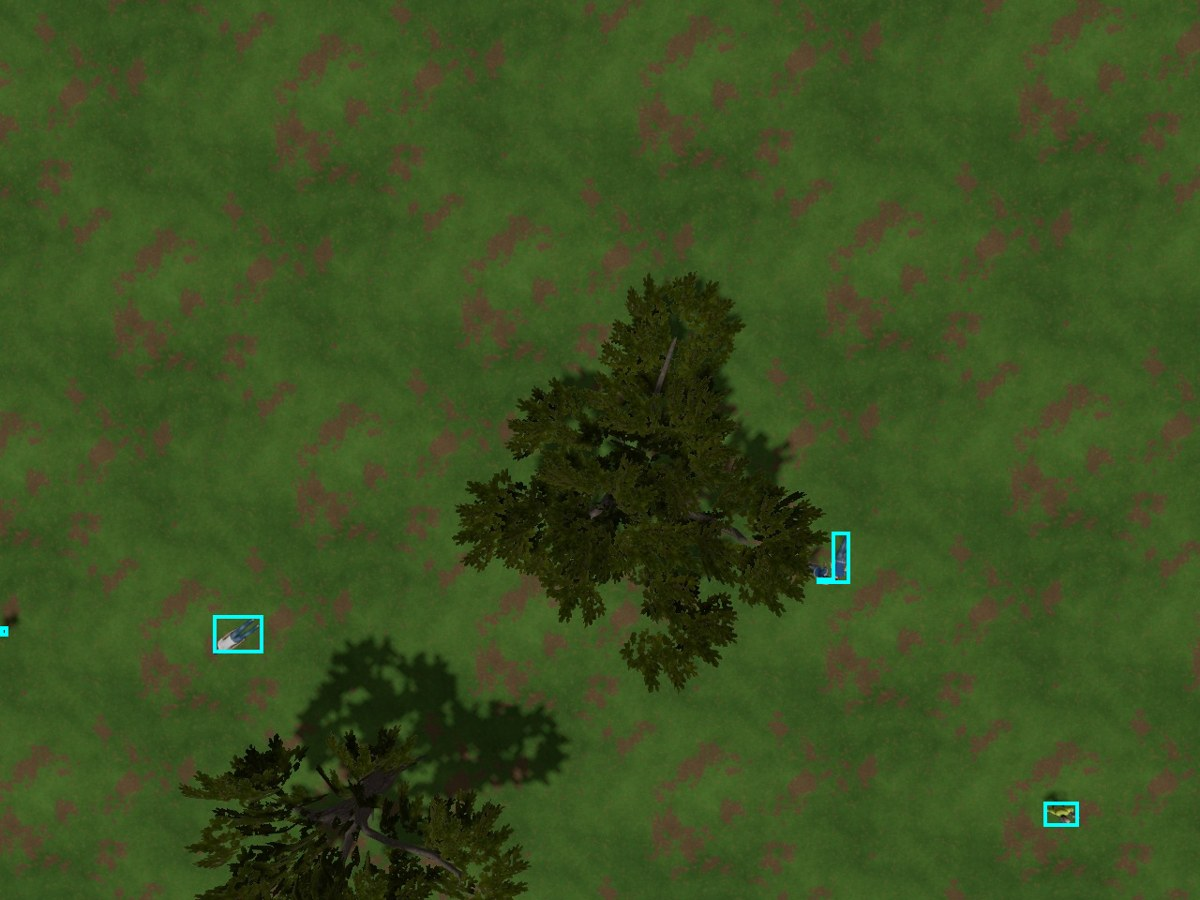
\includegraphics[width=0.8\textwidth]{dataset_etiquetas.jpg}
\caption{Una imagen del dataset con sus etiquetas automáticas (recuadros cian).}
\end{figure}

\section{Entrenamiento}

\begin{lstlisting}[style=bash]
~/.venvs/yolo/bin/python scripts/entrenar_detector.py entrenar --datos ~/datasets/personas_bosque/datos.yaml --epocas 80
\end{lstlisting}

Se parte de los pesos de YOLO26s preentrenados en COCO y se ajusta con imágenes de 1280 píxeles (sin
reducir: las personas son pequeñas) en la GPU. El mejor modelo se copia a
\cod{yolo/personas_yolo26s.pt}, que es el que usa la misión. Resultado en validación (300 imágenes):
\textbf{AP50 = 0.954}, AP50-95 = 0.692, precisión 0.96, recall 0.92, 15.6~ms por imagen.

\begin{figure}[H]
\centering
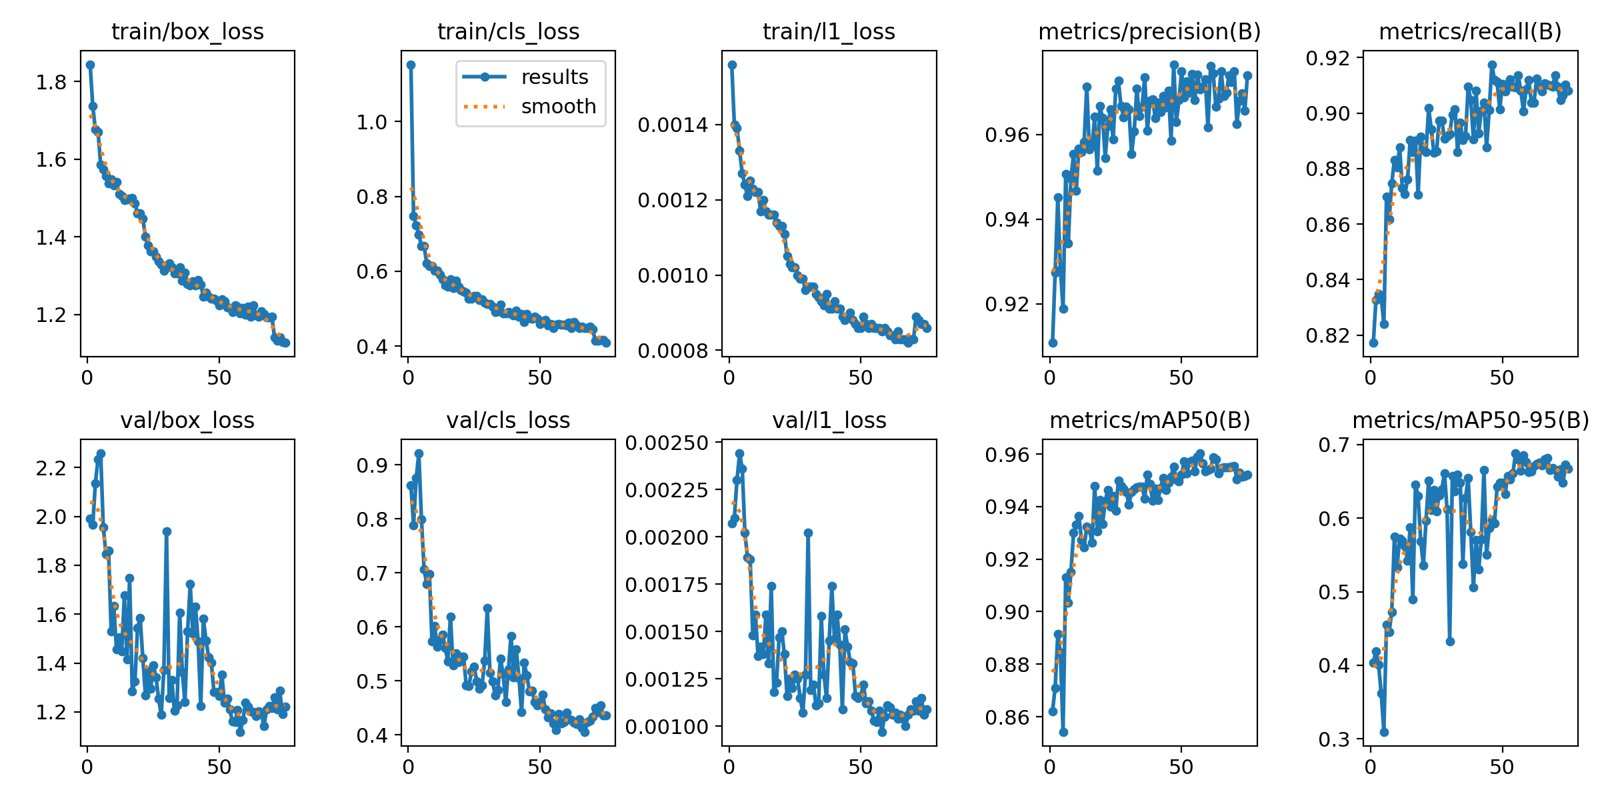
\includegraphics[width=\textwidth]{yolo_p_resultados.jpg}
\caption{Curvas de entrenamiento del detector de personas.}
\end{figure}

\begin{figure}[H]
\centering
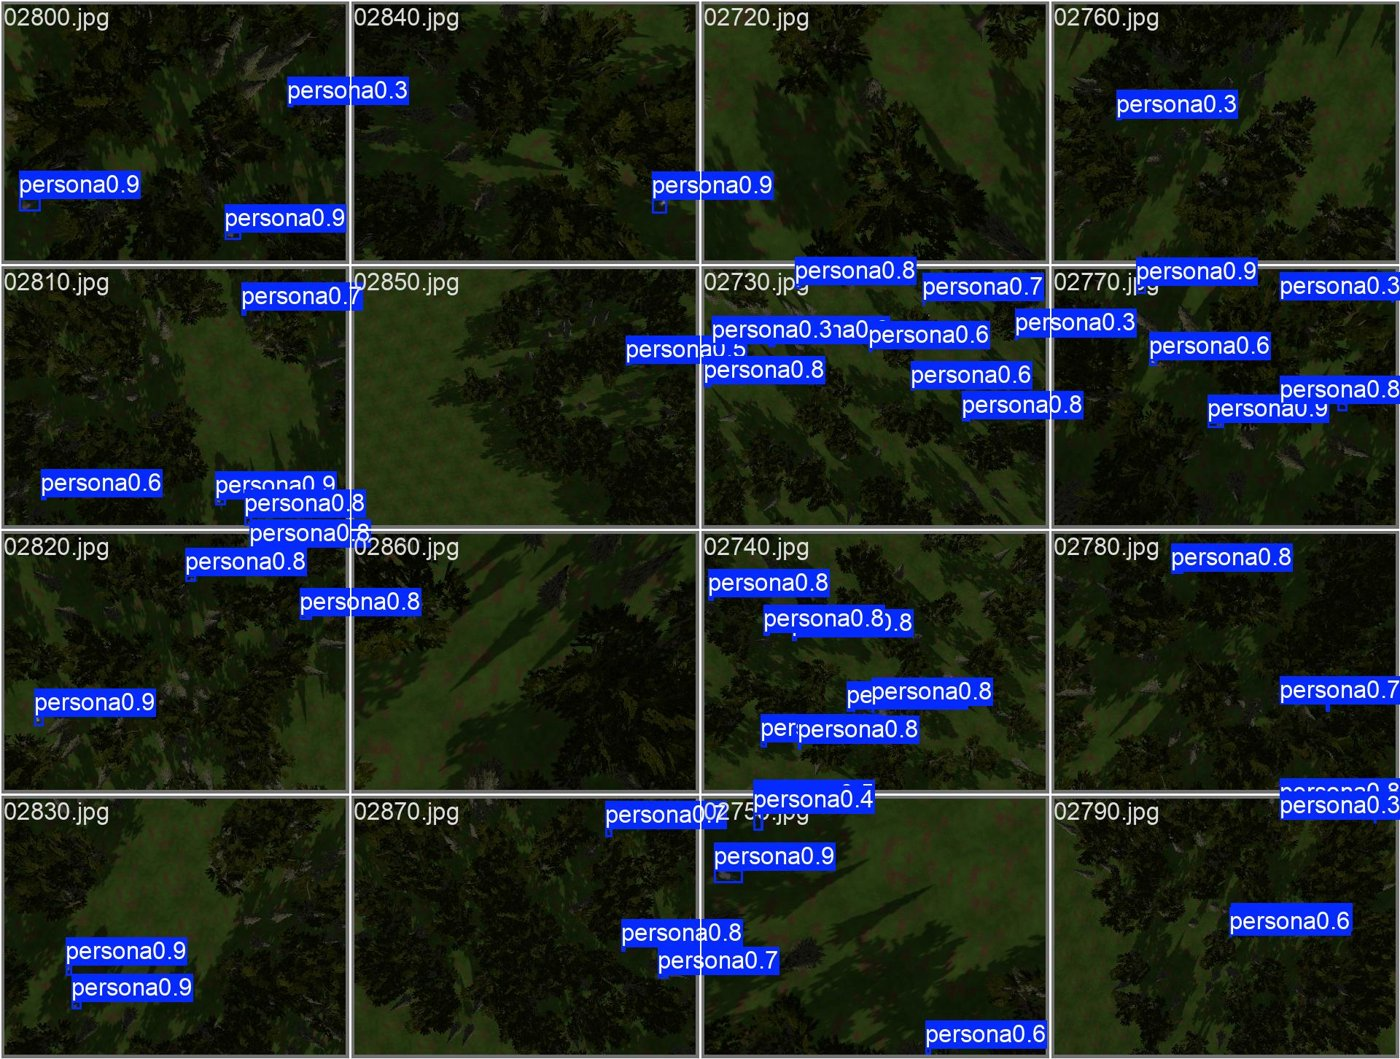
\includegraphics[width=0.85\textwidth]{yolo_p_pred.jpg}
\caption{Predicciones del detector sobre imágenes de validación.}
\end{figure}

\section{Por estrato: dónde falla}

\begin{figure}[H]
\centering
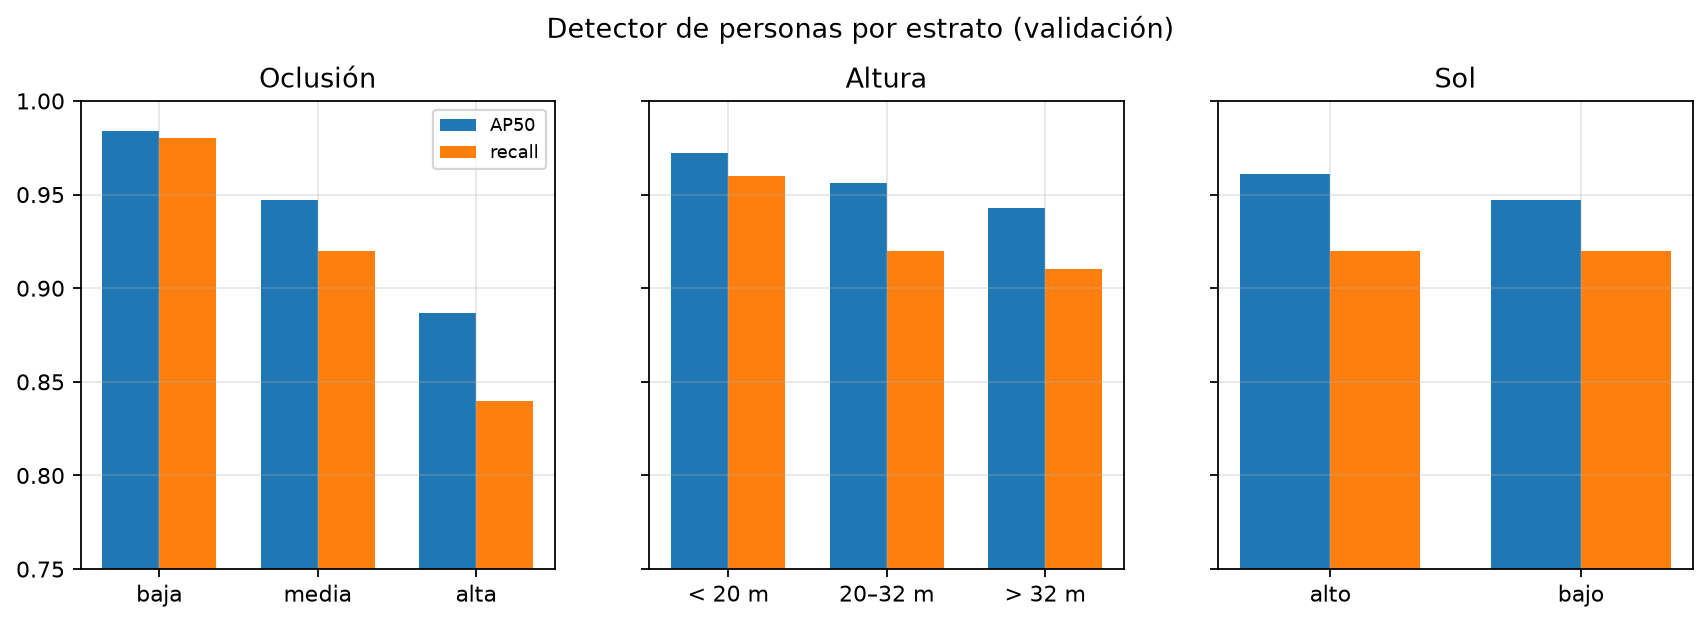
\includegraphics[width=\textwidth]{detector_estratos.png}
\caption{El detector pierde más personas con más copas (recall 0.98 $\rightarrow$ 0.84) y con más
altura; la iluminación casi no importa.}
\end{figure}

\begin{nota}
Con el YOLO26n preentrenado en COCO, sin ajustar, la misión localizó 0 de 3 personas: COCO casi no tiene
personas vistas desde arriba a 30~m. El ajuste con imágenes del simulador es indispensable; para el dron
real habrá que agregar imágenes reales (por ejemplo, el conjunto HERIDAL; \cod{scripts/preparar_datos.py}
las convierte).
\end{nota}

\section{El nodo detector}

\cod{mision/detector_node.py} corre con el Python de \cod{~/.venvs/yolo}, lee \cod{/camera}, aplica el
modelo y publica las cajas en \cod{/detecciones} (con la marca de tiempo de la imagen) y la imagen
anotada en \cod{/camera_yolo}, que Gazebo muestra en el panel ``Detección de personas''. Para estudiar
qué pasa si el detector es más lento (por ejemplo en una computadora a bordo), se le puede agregar
latencia (\cod{latencia_extra_ms}) o hacer que salte cuadros (\cod{saltar_cuadros}).
